\documentclass[10pt,a4paper]{report}
\usepackage[utf8]{inputenc}
\usepackage[spanish,es-tabla]{babel}
\usepackage{amsmath}
\usepackage{amsfonts}
\usepackage{amssymb}
\usepackage{graphicx}
\usepackage{wrapfig}
\usepackage{multirow}
\usepackage{float}
\usepackage{subfigure} 
\usepackage{pdflscape}
\usepackage{imakeidx}
\usepackage{fancyvrb}
\makeindex[columns=3, title=Alphabetical Index, intoc]
\usepackage{ragged2e}


\begin{document}
\begin{center}
	{\bf {\huge Instituto Tecnológico de Morelia} }\\ \vspace{1cm} 
	
\includegraphics[scale=.7]{logoITM.png} \hspace{6cm} 
\end{center}

\begin{center}
	\vspace{1cm}
	{\huge Practicas y Tareas} \vspace{1cm} \\
	{\bf {\Large Inteligencia Artificial}} \vspace{1cm} \\
	{\Large Haziel Josue Castillo Vazquez}\vspace{1cm} \\
	{\Large No. Control: 15120277} \vspace{2cm} \\
	{\Large Profesor: Alcaraz Chavez Jesus Eduardo}
\end{center}

\pagebreak 

\section*{Indice}
\begin{flushleft}
{\sc {\bf Introducción} \dotfill  3}\\
{\sc {\bf Contenido} \dotfill  4}\\ \hspace{.5cm}
	{\sc {\bf Practica 1. Heurística} \dotfill  4} \\ \hspace{1cm}
		{\sc Practica 1.1 Senku\dotfill  4}\\ \hspace{.5cm}
		

\end{flushleft}

\pagebreak 

\section*{Introducción}
Este documento se esta realizando con el fin de documentar practicas, tareas individuales y en equipo de la materia de Inteligencia Artificial.\\ 

\pagebreak 

\section*{Contenido}
\section*{Practica 1. Heurística}
{\sc {\bf Practica 1.1.-  Senku}}\\

Senku (en inglés "Peg Solitaire" o "Sailor's Solitaire") es un juego para un solo jugador muy popular ya que juega con un tablero que tiene una serie de agujeros en el patrón de un signo de más. Hay clavija para todos los orificios excepto uno.\\

\begin{center}
	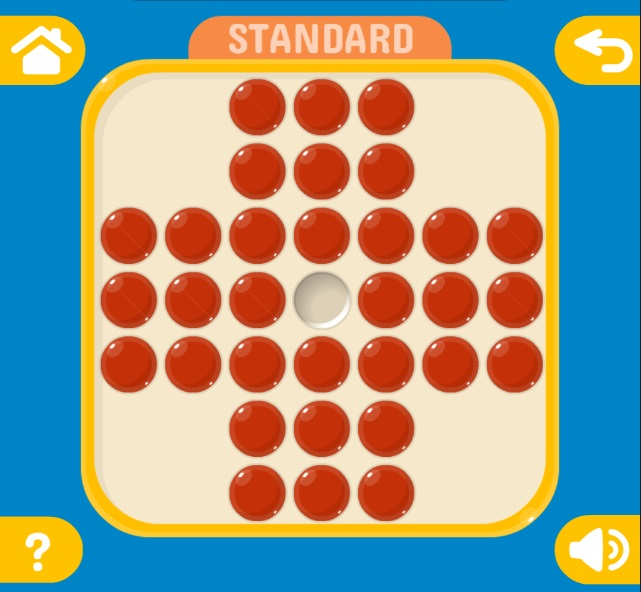
\includegraphics[scale=.3]{initialState.jpg} \hspace{6cm} 
\end{center}

El objetivo es limpiar el tablero de todas las clavijas, excepto uno. Un "salto" consiste en mover una ficha en línea recta sobre cualquier ficha adyacente para aterrizar sobre la siguiente casilla vacía, en sentido izquierda-derecha o arriba-abajo, nunca en diagonal. La ficha sobre la que se ha saltado se retira del tablero. \\

\begin{center}
	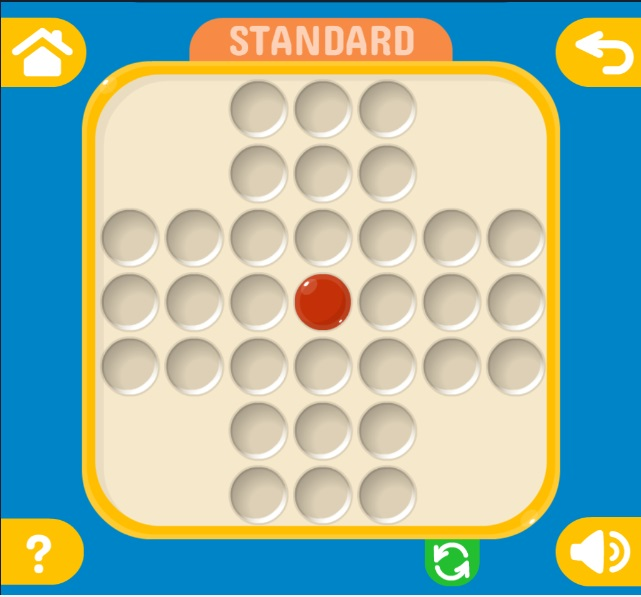
\includegraphics[scale=.3]{finalState.jpg} \hspace{6cm} 
\end{center}

\pagebreak 
El algoritmo tiene como primer objetivo limpiar las extremidades del tablero.

\begin{center}
	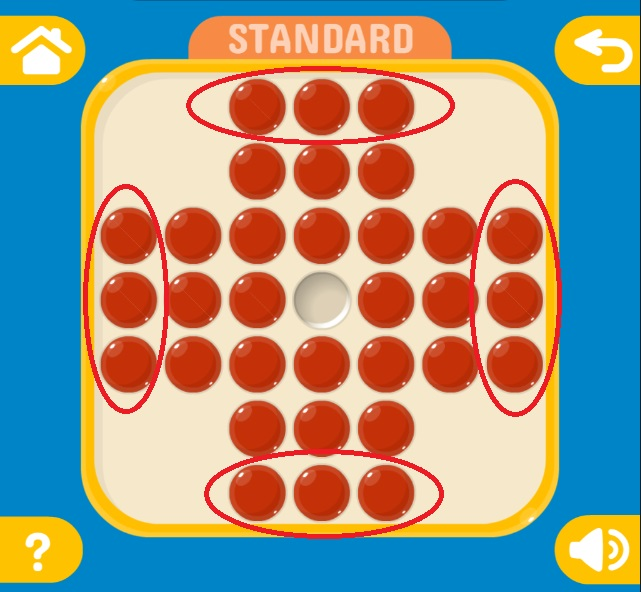
\includegraphics[scale=.3]{1.jpg} \hspace{6cm} 
\end{center}

Podemos comenzar con cualquier extremidad ya que el tablero es simétrico, así que en nuestro caso elegiremos la parte inferior. Ahora bien, para limpiar cualquier extremo lo hacemos
de derecha a izquierda.

\begin{center}
	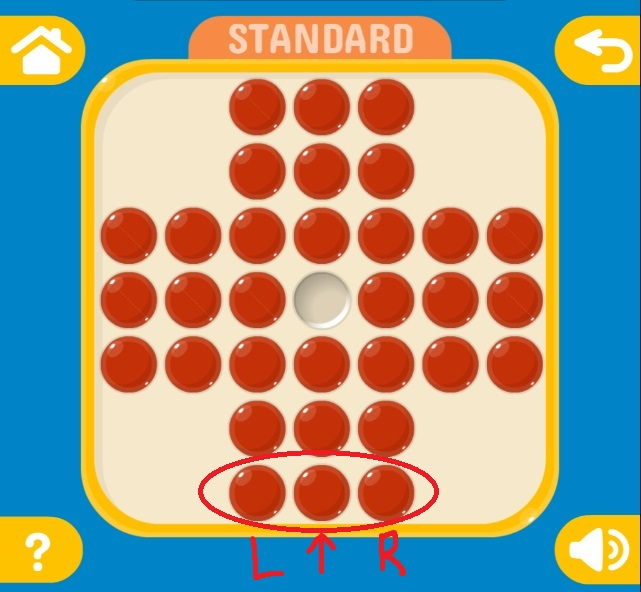
\includegraphics[scale=.3]{2.jpg} \hspace{6cm} 
\end{center}

\pagebreak 

Como podemos observar en la imagen de abajo, no se puede simplemente limpiar la posición inferior derecha porque no es un movimiento valido, ya que la posición a la que lo queremos mover esta ocupada, así que tenemos que despejar esa posición para poder permitirle el movimiento. Tomamos la posición de la derecha he intentamos limpiar el centro brincando hacia la izquierda, pero podemos observar que nuevamente esa posición esta ocupada, así que ahora nuestro objetivo es limpiar esa nueva posición.


\begin{center}
	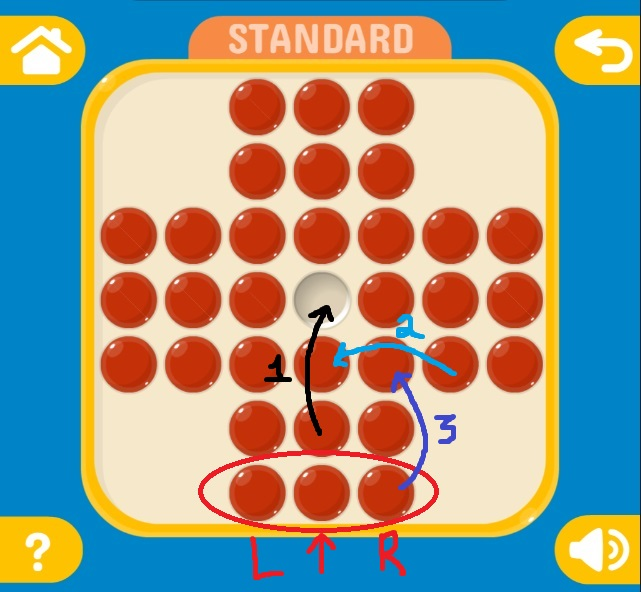
\includegraphics[scale=.3]{3.jpg} \hspace{6cm} 
	
	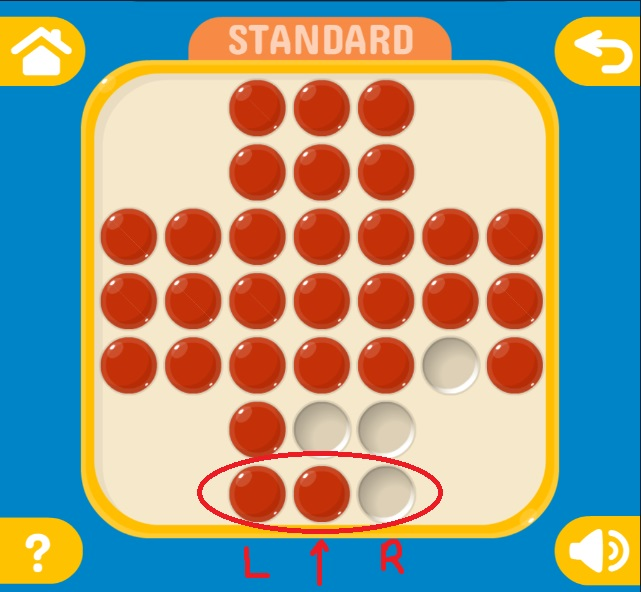
\includegraphics[scale=.3]{4.jpg} \hspace{6cm} 
\end{center}
\pagebreak 
Ya hemos limpiado la primer posicion de la derecha, ahora continuamos con la posicion central. Tomamos la posicion a su izquierda y brincamos a la derecha

\begin{center}
	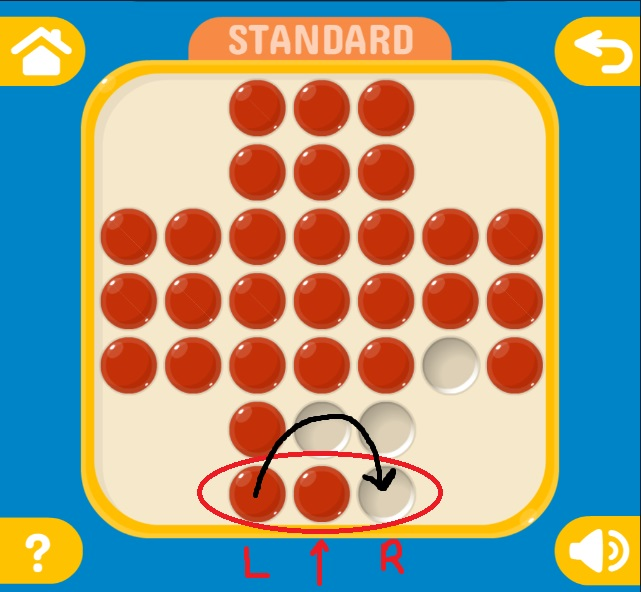
\includegraphics[scale=.3]{5.jpg} \hspace{6cm}
	
	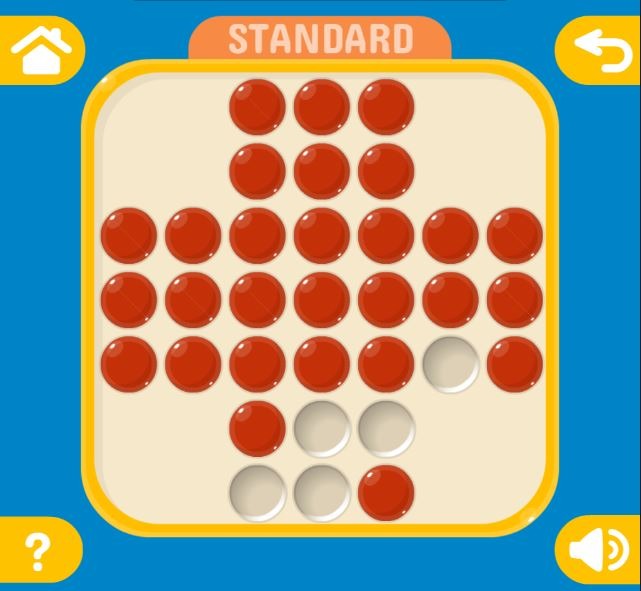
\includegraphics[scale=.4]{6.jpg} \hspace{6cm} 
\end{center}
\pagebreak 
Volvemos a tener una pieza en la posición inferior derecha, tenemos que moverla hacia arriba
pero esta ocupada esa posición, por lo que tenemos que limpiarla para poder hacer el salto.

\begin{center}
	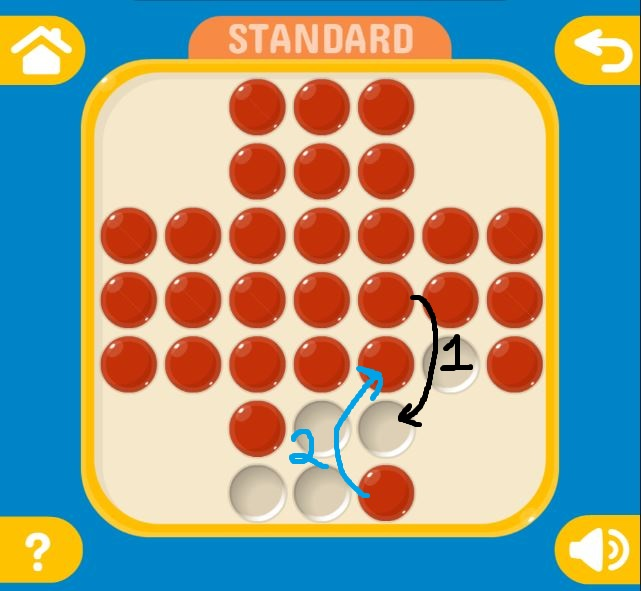
\includegraphics[scale=.3]{7.jpg} \hspace{6cm} 
	
	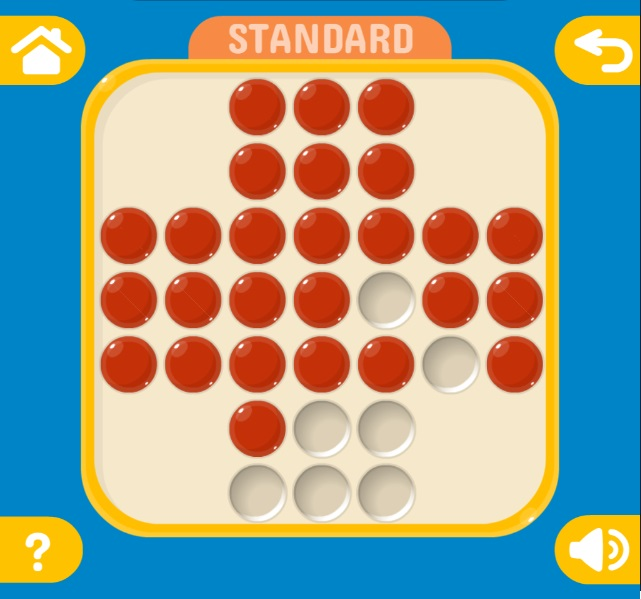
\includegraphics[scale=.3]{8.jpg} \hspace{6cm}
\end{center}

\pagebreak
Ahora rotamos el tablero (nuestra matriz en el codigo) y comenzamos de nuevo a limpiar la parte inferior repitiendo los mismos pasos anteriores para cada area.

\begin{center}
	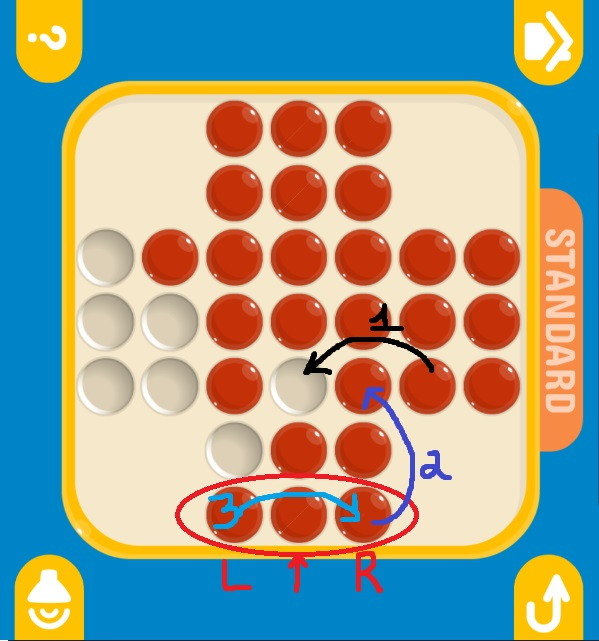
\includegraphics[scale=.3]{10.jpg} \hspace{6cm}
	
	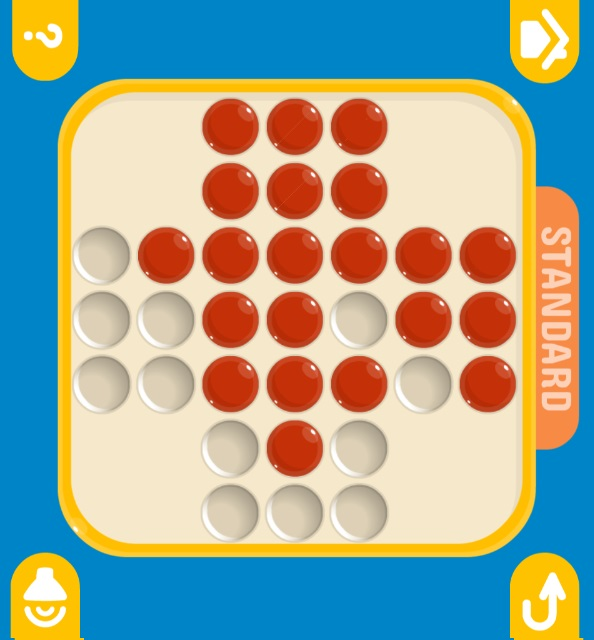
\includegraphics[scale=.3]{11.jpg} \hspace{6cm}
	
	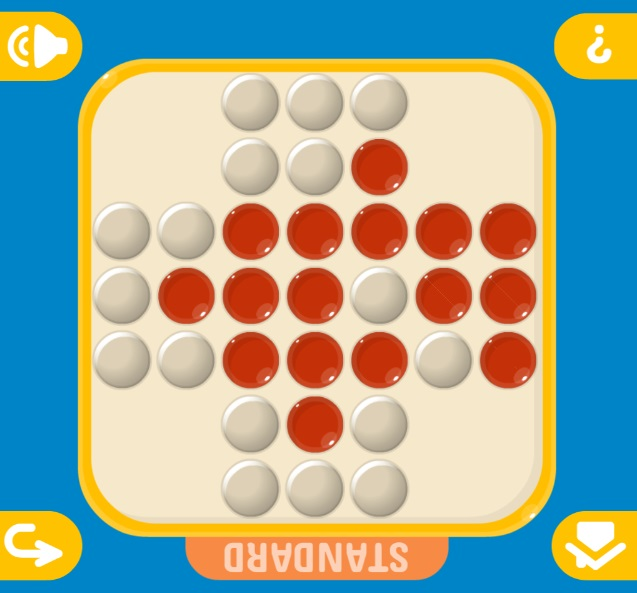
\includegraphics[scale=.3]{12.jpg} \hspace{6cm}
	
	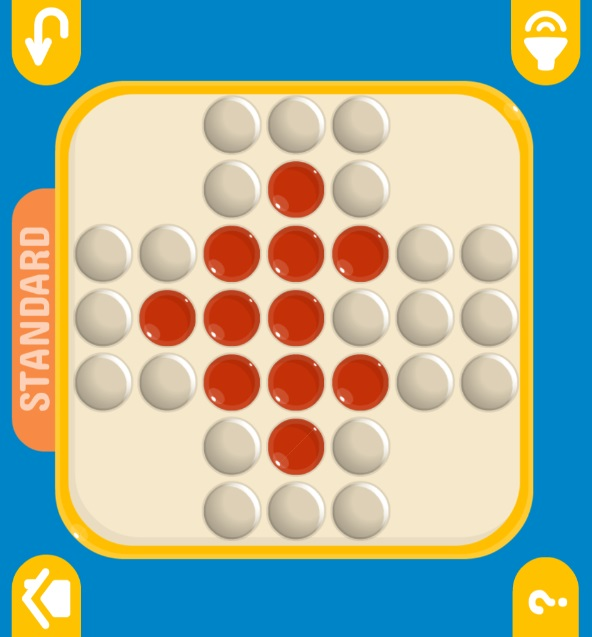
\includegraphics[scale=.3]{13.jpg} \hspace{6cm}
\end{center}

Ahora tenemos una forma parecida a una flecha apuntando hacia arriba o a la forma de una casa.
\begin{center}
	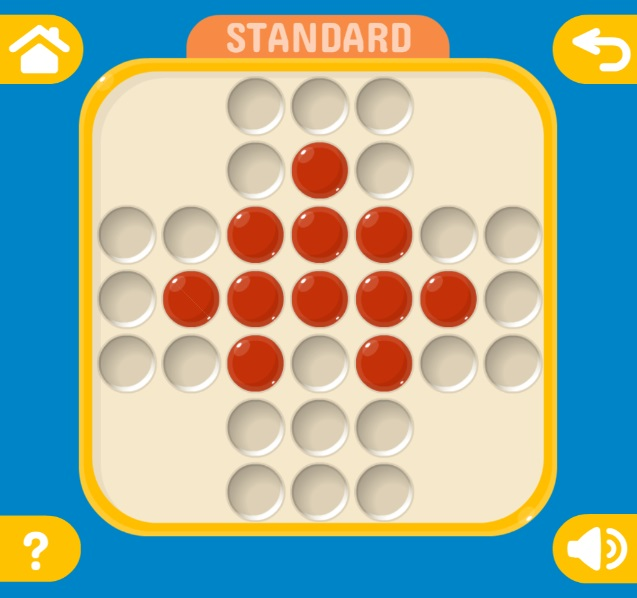
\includegraphics[scale=.3]{14.jpg} \hspace{6cm}
\end{center}

Realizamos la siguiente secuencia hasta formar una "T invertida".

\begin{center}
	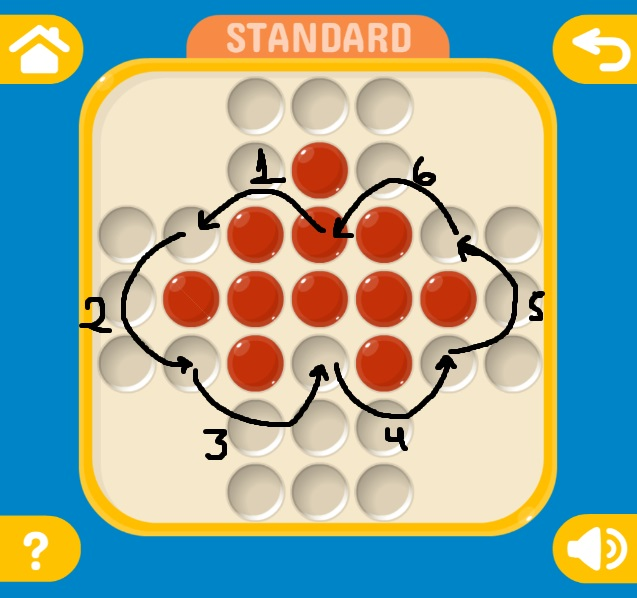
\includegraphics[scale=.3]{15.jpg} \hspace{6cm}
	
	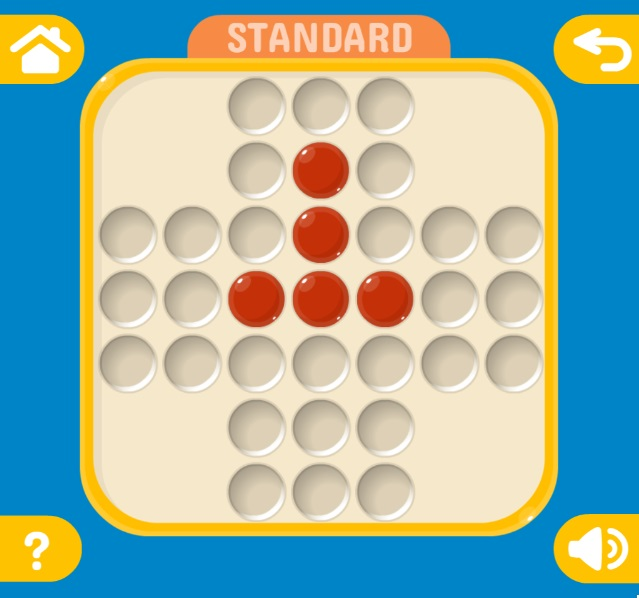
\includegraphics[scale=.3]{16.jpg} \hspace{6cm}
\end{center}

Terminamos eliminando las extremidades de la "T invertida"

\begin{center}
	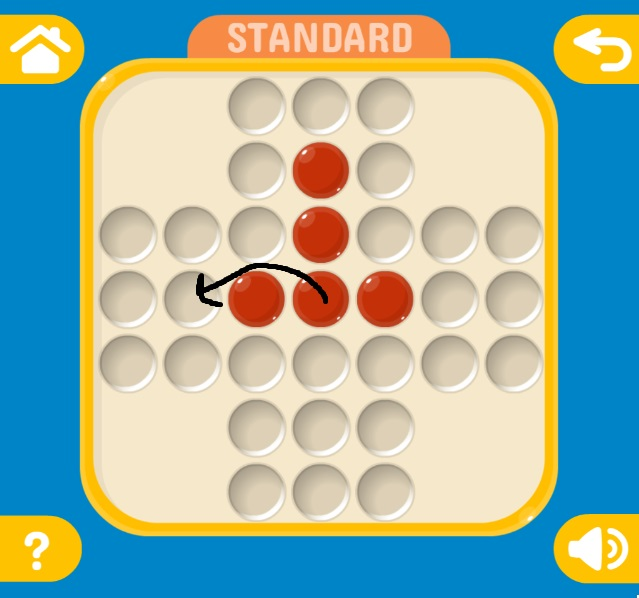
\includegraphics[scale=.3]{17.jpg} \hspace{6cm}
	
	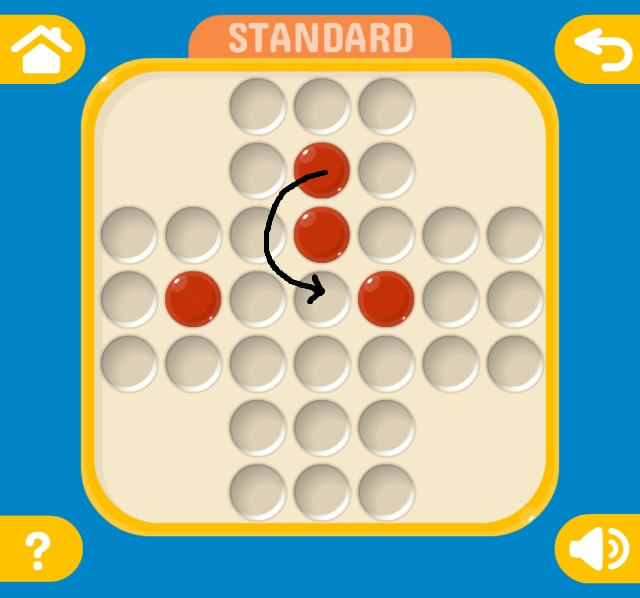
\includegraphics[scale=.3]{18.jpg} \hspace{6cm}
	
	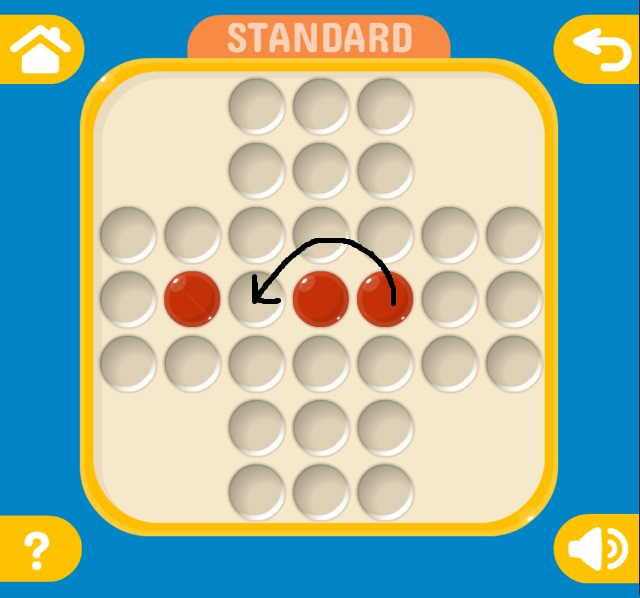
\includegraphics[scale=.3]{19.jpg} \hspace{6cm}
	
	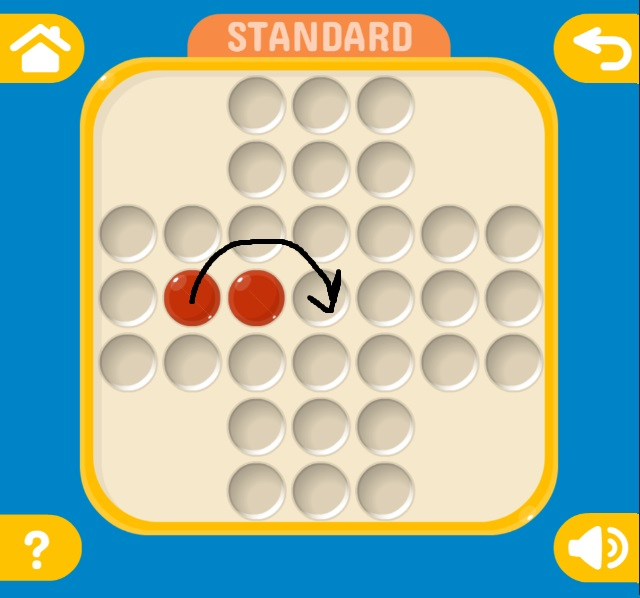
\includegraphics[scale=.3]{20.jpg} \hspace{6cm}
	
	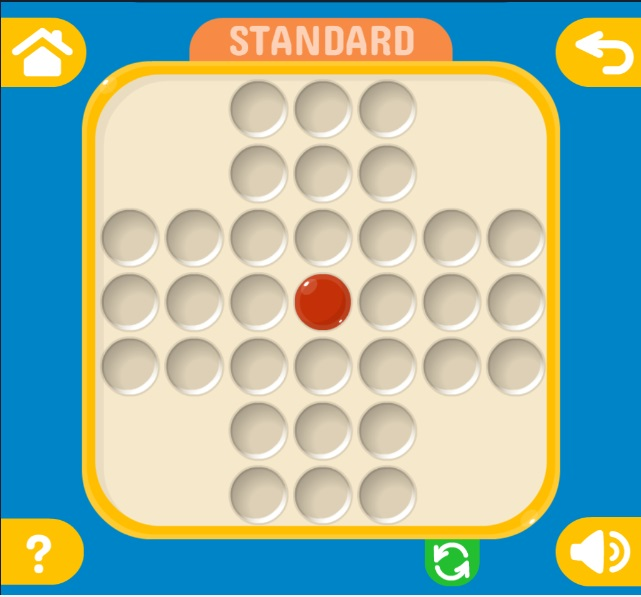
\includegraphics[scale=.3]{finalState.jpg} \hspace{6cm}
\end{center}

Ya fue explicado el algoritmo, ahora se mostrara el codigo con sus respectivas impresiones paso por paso

\begin{Verbatim}[tabsize=4]
/*
Defino una array 7 x 7 que representa mi tablero Zenku (Peg)

*  Los numeros 2 son posiciones que no podemos operar
*  Los numeros 1 son posiciones que estan ocupadas
*  Los numeros 0 son posiciones que estan vacias
*/
let array = [
	[2,2,1,1,1,2,2],
	[2,2,1,1,1,2,2],
	[1,1,1,1,1,1,1],
	[1,1,1,0,1,1,1],
	[1,1,1,1,1,1,1],
	[2,2,1,1,1,2,2],
	[2,2,1,1,1,2,2]
]

function printArray() {
	for (let i = 0; i < array.length; i++) {
		console.log(array[i]);        
	}
	console.log("\n")
}

function cleanBottom(){
	printArray()

	if(array[6][4] === 1){
		if(array[4][4] === 1){
			if(array[4][3] === 1) {
				if(array[3][3] === 0) {
					array[3][3] = 1
					array[4][3] = 0
					array[5][3] = 0
					
					cleanBottom()
				} else {
					array[3][4] = 0
					array[4][4] = 0
					array[5][4] = 1
					
					cleanBottom()
				}
			} else {
				array[4][3] = 1
				array[4][4] = 0
				array[4][5] = 0
				
				cleanBottom()
			}
		} else {
			array[4][4] = 1
			array[5][4] = 0
			array[6][4] = 0
		
			cleanBottom()
		}
	} else if(array[6][2] === 1 && array[6][4] === 0) {
		array[6][2] = 0
		array[6][3] = 0
		array[6][4] = 1
	
		cleanBottom()
	}

}

function rotateRightMatrix() {
	// Declaro una matriz auxiliar
	let aux = [
	[0,0,0,0,0,0,0],
	[0,0,0,0,0,0,0],
	[0,0,0,0,0,0,0],
	[0,0,0,0,0,0,0],
	[0,0,0,0,0,0,0],
	[0,0,0,0,0,0,0],
	[0,0,0,0,0,0,0],
	]

	// Calculamos la transpuesta
	for (let i = 0; i < array.length; i++) {
		for (let j = 0; j < array.length; j++) {
			aux[j][i] = array[i][j]
		}
	}

	// Hacemos reverse a los elementos de cada fila
	for (let i = 0; i < array.length; i++) {
		aux[i].reverse()
	}
	array = aux
} 

function cleanAllSides(){
	// Si hay por lo mens un 1 en la parte inferior central de la matriz
	if(array[6][2] === 1 || array[6][3] === 1 || array[6][4] === 1) {
		cleanBottom() // Limpiamos la zona inferior
		rotateRightMatrix() // Rotamos la matriz a la derecha
		cleanAllSides() // Volvemos a llamar a la funcion
	} 
}

function main(){
	cleanAllSides() // Limpia todas las extremidades
	printArray()
}

main() // Ejecutamos la funcion principal
\end{Verbatim}



\end{document}
